\beginsong{Clementine}
\beginverse
In a cavern, in a canyon,
excavating for a mine,
dwelt a miner, fortyniner, 
and his daughter, Clementine.
\endverse
\beginchorus
Oh my darling, oh my darling,
oh my darling, Clementine.
You are lost and gone forever,
dreadful sorry, Clementine.
\endchorus
\beginverse
Light she was, and like a fairy,
and her shoes were number nine,
Herring boxes, without topses,
sandals were for Clementine.
\endverse
\beginverse
Drove she ducklings to the water,
ev’ry morning, just at nine
hit her foot against a splinter,
fel into the foaming brine.
\endverse
\beginverse
Ruby lips above the water,
blowing bubbles, soft and fine,
but alas, I was no swimmer, 
so I lost my clementine.
\endverse
\beginverse
In a corner of the churchyard,
Where the myrtle boughs entwine,
Grow the roses in their poses,
Fertilized by Clementine.
\endverse
\beginverse
When the miner forty-niner,
Soon began to peak and pine,
Thought he oughter join his daughter,
Now he's with his clementine.
\endverse
\beginverse
In my dreams she still doth haunt me
robed in garments, soaked in brine,
though in life I used to hug her, 
now she’s dead I draw the line.
\endverse
\beginverse
How I missed her, how I missed her
How I missed my Clementine.
So I kissed her little sister,
And forgot my Clementine.
\endverse
\endsong
\begin{intersong}
    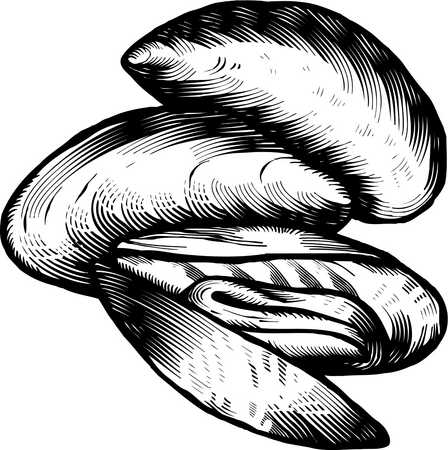
\includegraphics[width=0.4\textwidth]{cocklesandmussels}
\end{intersong}